%%%%%%%%%%%%%%%%%%%%%%%%%%%%%%%%%%%%%%%%%%%%%%%%%%%%%%%%%%%%%%%%%%%%
\section{Interfaces}
\label{sec:fdsp-apa-intfc}

The interface between the \dword{apa} consortium and other detector consortia, facilities, and working groups covers a wide range of activities. Table~\ref{tab:apa_interface_docdb} summarizes the interface control documents under development. In the following sections, we elaborate slightly on the interfaces with the \dword{tpc} readout electronics and the \dword{pds}, as well as the cable routing plan for both systems.  Other important interfaces are to the \dword{tpc} \dword{hv} system (the \dword{fc}) and the \dword{dss} inside the \dword{dune} cryostats.  

\begin{dunetable}
[APA Interface Links]
{p{0.4\textwidth}p{0.2\textwidth}}
{tab:apa_interface_docdb}
{\dword{apa} Interface Links. %\forlbnc{These DocDB links will be updated to EDMS links before final TDR version.}
%\fixme{no, we will freeze a copy in docdb for the TDR, future updates beyond the TDR will go to EDMS. anne}
}
Interfacing System & Linked Reference \\ \toprowrule
TPC electronics & \citedocdb{6670} \\ \colhline 
Photon detector system & \citedocdb{6667} \\ \colhline
Drift high voltage system & \citedocdb{6673} \\ \colhline
DAQ & \citedocdb{6676} \\ \colhline
Slow controls and cryogenics & \citedocdb{6679} \\ \colhline
Integration facility & \citedocdb{7021} \\ \colhline
Facility interfaces %(Detector Hall, Cryostat, and Cryogenics) 
& \citedocdb{6967} \\ \colhline
Installation & \citedocdb{6994} \\ \colhline
Calibration & \citedocdb{7048} \\ \colhline
Software computing & \citedocdb{7102} \\ \colhline
Physics & \citedocdb{7075} \\
%CISC & \citedocdb{6787}{1} \\ \colhline
%... & \citedocdb{nnnn}{n} \\ \colhline
%(last item)& \citedocdb{}{} \\
\end{dunetable}

\begin{comment}
\begin{dunetable}[APA interface control documents]{lr}{tab:apa_interface_docdb}
{Summary of interface control documents being developed.}  
  Interface Document & DUNE DocDB number \\\colhline 
  Interface to TPC electronics & 6670 \\ \colhline 
  Interface to photon detector system & 6667 \\ \colhline
  Interface to drift high voltage system & 6673 \\ \colhline
  Interface to DAQ & 6676 \\ \colhline
  Interface to slow controls and cryogenics infrastructure & 6679 \\\specialrule{1.5pt}{1pt}{1pt}
  Integration facility interface & 7021 \\ \colhline
  Facility interfaces (Detector Hall, Cryostat, and Cryogenics) & 6967 \\ \colhline
  Installation interface & 6994 \\ \colhline
  Calibration interface & 7048 \\\specialrule{1.5pt}{1pt}{1pt}
  Software computing interface & 7102 \\ \colhline
  Physics interface & 7075 \\ \colhline
\end{dunetable}
\end{comment}


%%%%%%%%%%%%%%%%%%%%%%%%%%%%%%%%%%%%%%%%%%%%%%%%%
\subsection{TPC Cold Electronics}
\label{sec:fdsp-apa-intfc-elec}

The \dword{tpc} readout electronics are directly mounted to the \dword{apa} immersed in \dword{lar} to reduce the input capacitance and thus inherent electronic noise.  With the wire-wrapped design, all \num{2560} wires to be read out (recall \num{960} are $G$-plane wires used for charge shielding only and so are not read out) terminate on wire boards that stack along one end (the head) of the \dword{apa} frame.  The \num{2560} channels are read out by \num{20} \dword{fe} motherboards (\num{128} channels per board), each of which includes eight \num{16}-channel \dword{fe} ASICs, eight \num{16}-channel \dword{adc} \dwords{asic}, \dword{lv} regulators, and input signal protection circuits.  Figure~\ref{fig:apa_ce} provides a schematic view of the head end of an \dword{apa} with electronics installed and a cable tray mounted above. 

\begin{dunefigure}[APA interface with TPC electronics]{fig:apa_ce}
{The head region of an \dword{apa} frame showing the ten wire board stacks on each side, \num{20} \dword{femb} boxes, and the cable tray mounted above.}
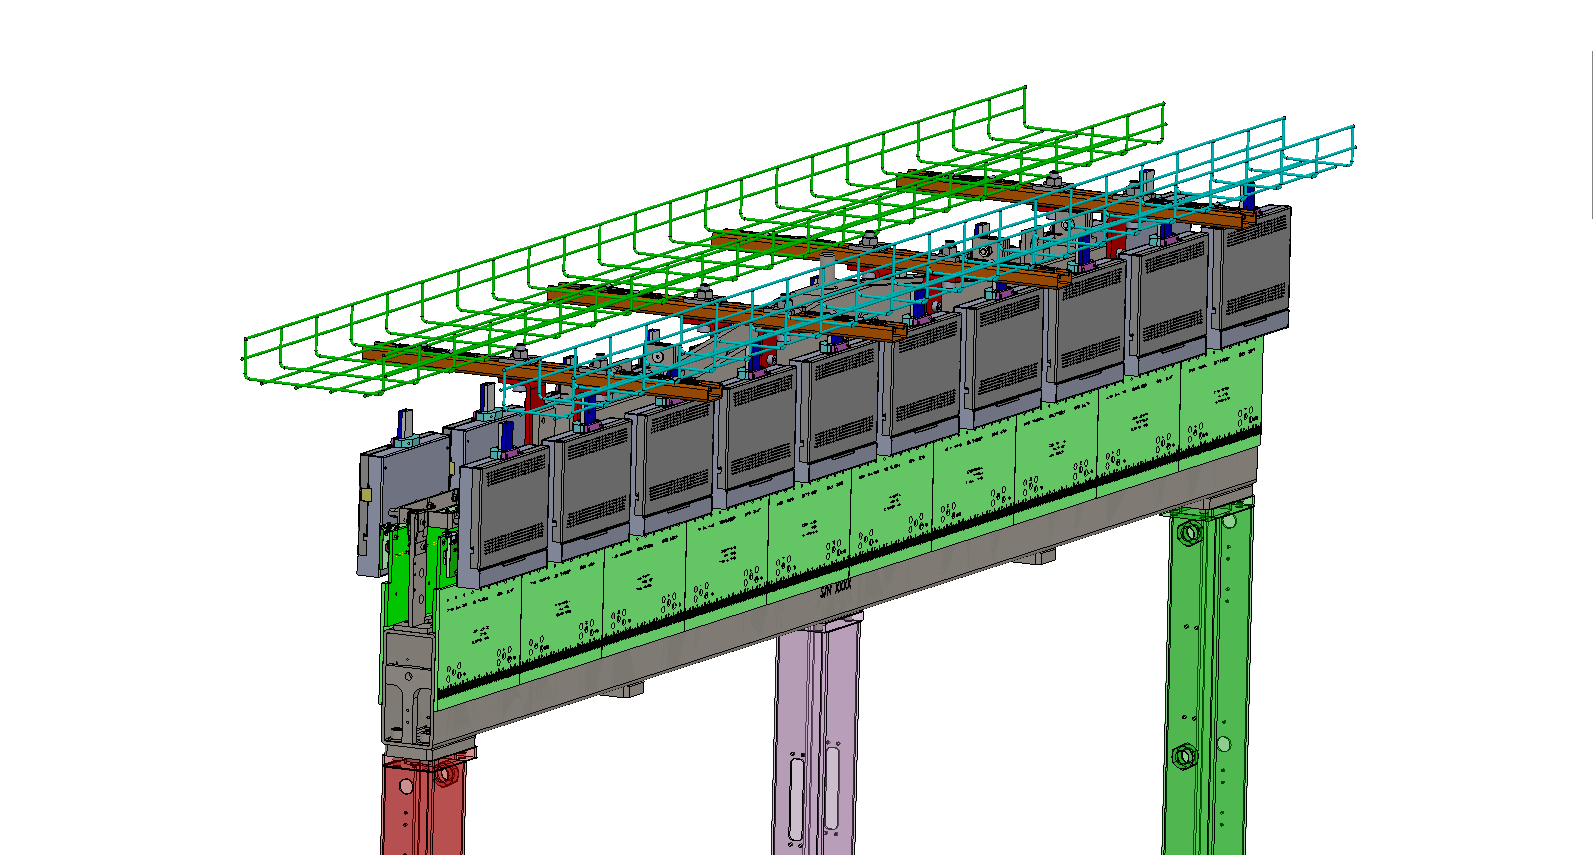
\includegraphics[width=0.85\textwidth,trim=10mm 0mm 10mm 20mm, clip]{sp-apa-elec-interface.png}
\end{dunefigure}

%The interface between the \dword{apa} and TPC \dword{ce} involves a wide range of topics, including the hardware design and production, testing, integration, installation, and commissioning. The hardware interface has two basic components: mechanical and electrical. 
The mechanical interface includes the support of the \num{20} \dword{ce} boxes, each housing a \num{128} channel \dword{femb}.  They are the gray, vertically oriented boxes  in Figure~\ref{fig:apa_ce}. 

The electrical interface covers the choice of wire-bias voltages to the four wire planes so that \num{100}\% transparency can be achieved for drifting ionization electrons, cable connection for the wire bias voltages from the cryostat feedthroughs to the \dword{cr} boards, interface boards connecting \dword{cr} boards and \dword{ce} boxes, filtering of wire-bias voltages through \dword{cr} boards to suppress potential electronic noise, and an overall grounding scheme and electrical isolation scheme for each \dword{apa}. The last item is particularly important to achieve the required low electronic noise levels.  See Chapter~\ref{ch:fdsp-tpc-elec} for information on all parts of the \dword{fe} electronics system.


%%%%%%%%%%%%%%%%%%%%%%%%%%%%%%%%%
\subsection{Photon Detection System}
\label{sec:fdsp-apa-intfc-pds}

The \dword{pds} is integrated into the \dword{apa} frame to form a single unit for detecting both ionization charge and scintillation light.  The \dword{apa} frame design must also accommodate cables for the photon detectors.  %Figure~\ref{fig:apa-pd} shows the interface for a light-guide bar based \dword{pds} like that deployed in \dword{pdsp}. 
Individual \dword{pd} units are inserted through \num{10} slots machined in the side steel tubes of the frame and supported by rails mounted in the \dword{apa}. Figures~\ref{fig:apa-frame-full} and \ref{fig:apa-frame-details} show examples of these features in the frame. Figure~\ref{fig:apa-pd} shows a \dword{pd} module being inserted into a slot in the frame and mating with an electrical connector mounted along the center tube in the \dword{apa}.

\begin{dunefigure}[APA interface with PDs in ProtoDUNE-SP]{fig:apa-pd}
{Top: A \dword{pd} module in \dword{pdsp} being inserted into a slot in the frame. Bottom: The \dword{pd} unit mating with an electrical connector mounted along the center tube in the \dword{apa}.
%Installation of a \dword{pds} module into the available slots in the \dword{apa} frame. %Also shown is a concept for routing \dword{pds} cables through the rib tubes of the \dword{apa} frame and up the central vertical tube section.
}
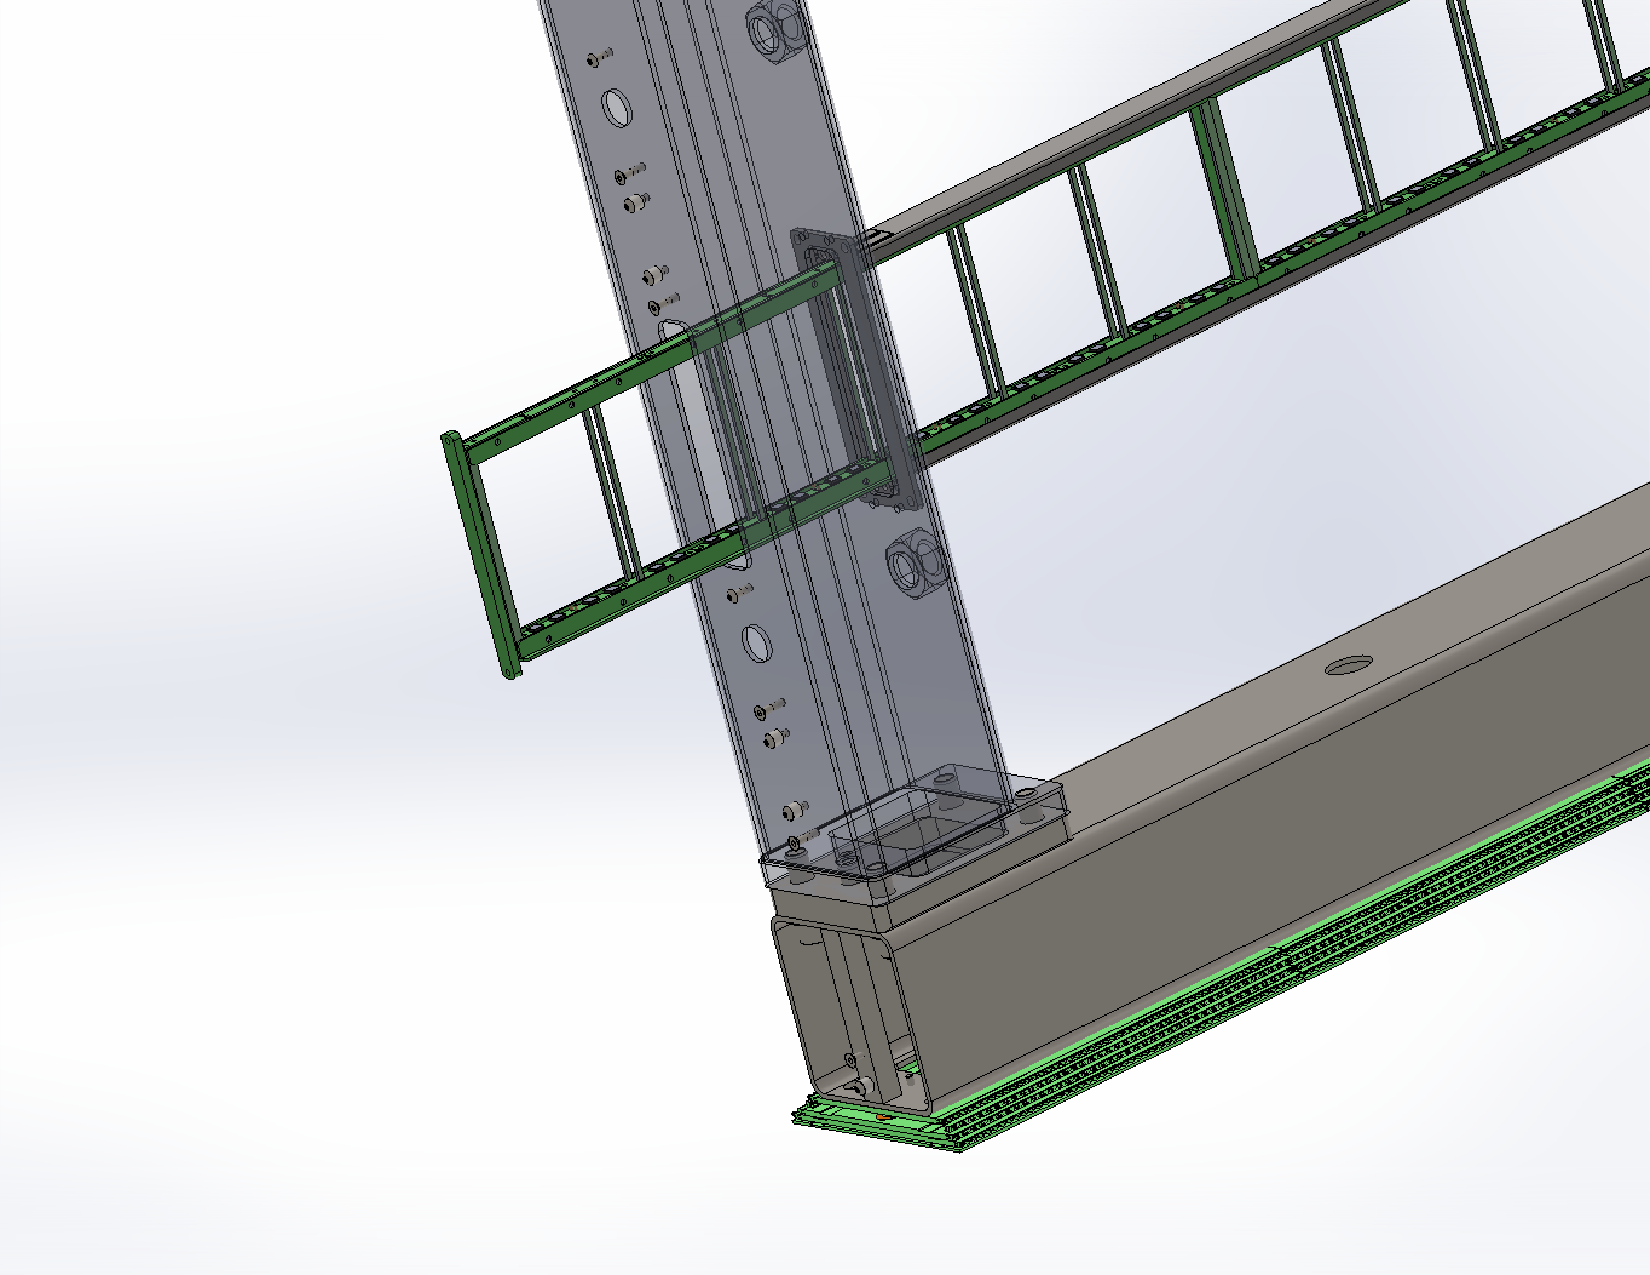
\includegraphics[height=0.4\textheight,trim=0mm 0mm 0mm 0mm,clip]{sp-apa-pds-module-insertion-in-frame.pdf}\\
\vspace{2mm}
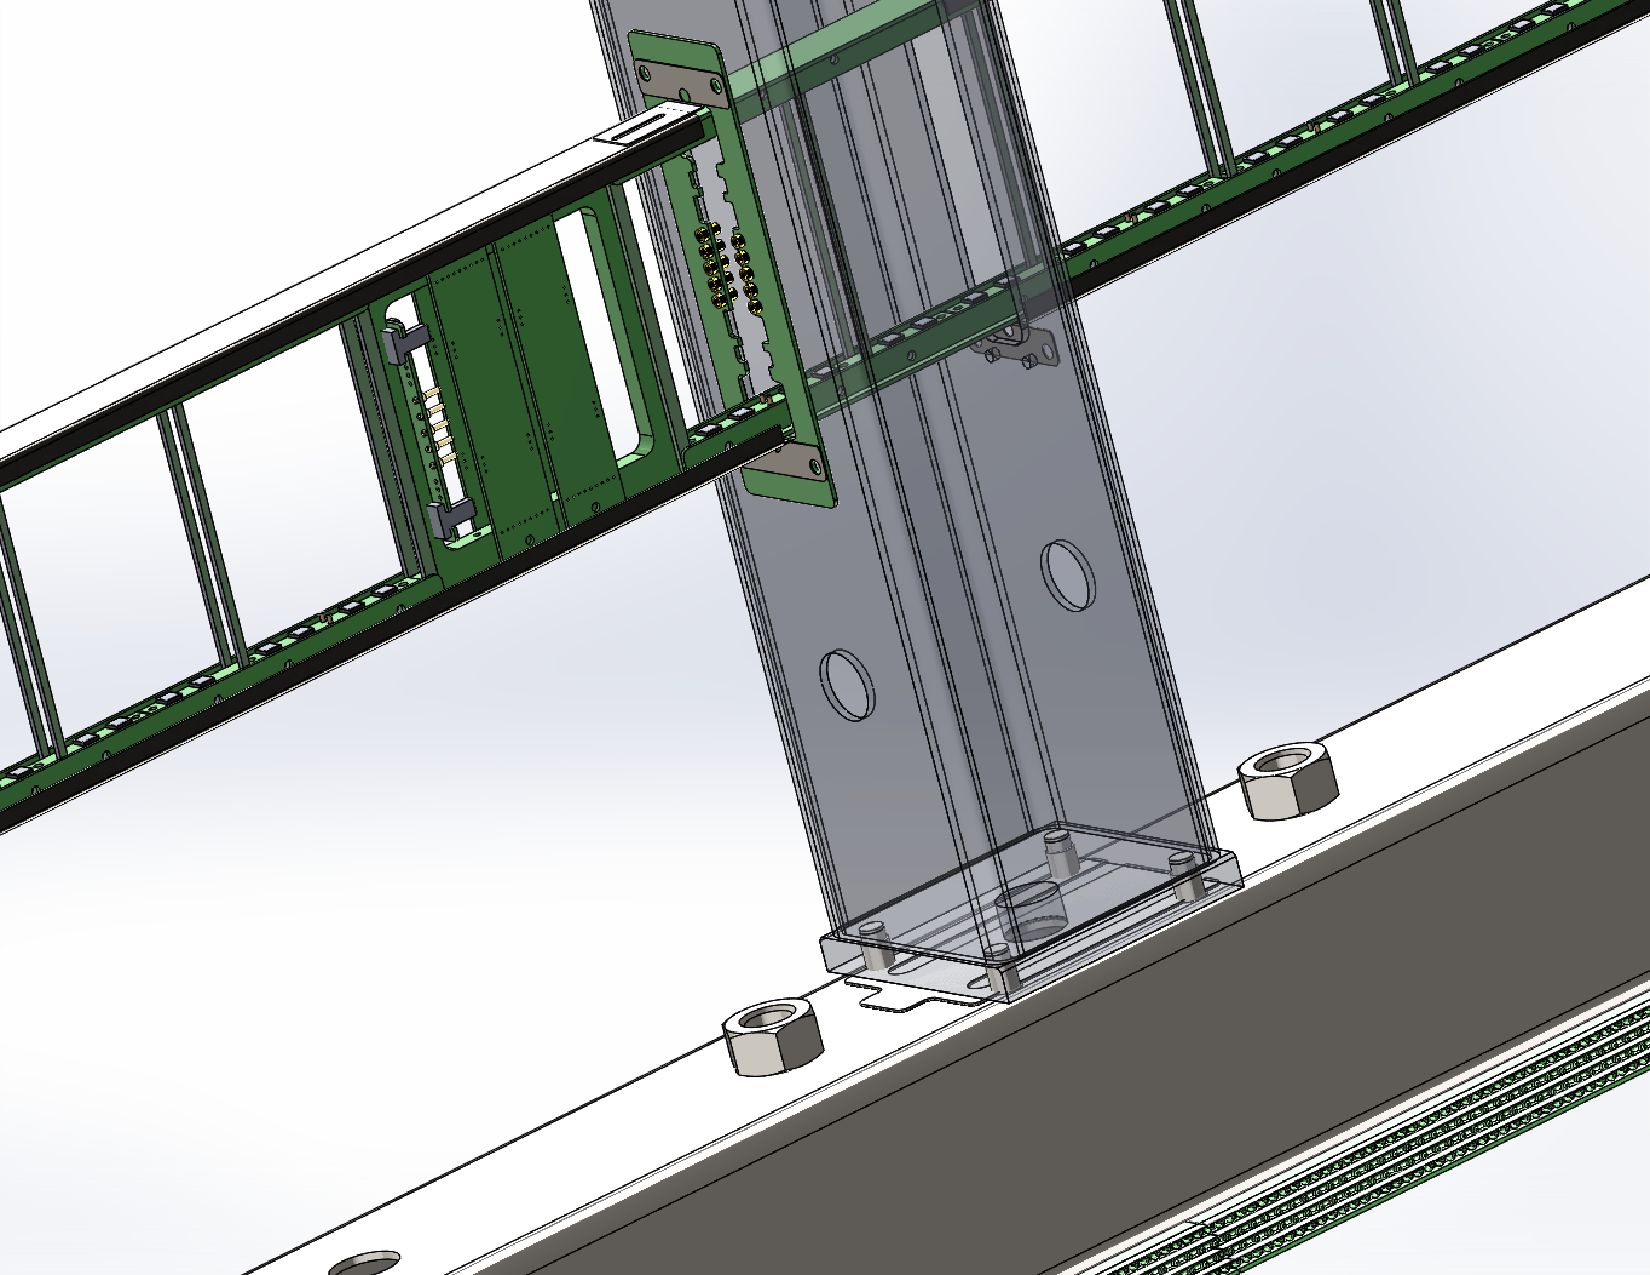
\includegraphics[height=0.4\textheight,trim=0mm 0mm 0mm 0mm,clip]{sp-apa-pds-center-tube-insertion.pdf}
%\qquad\qquad
%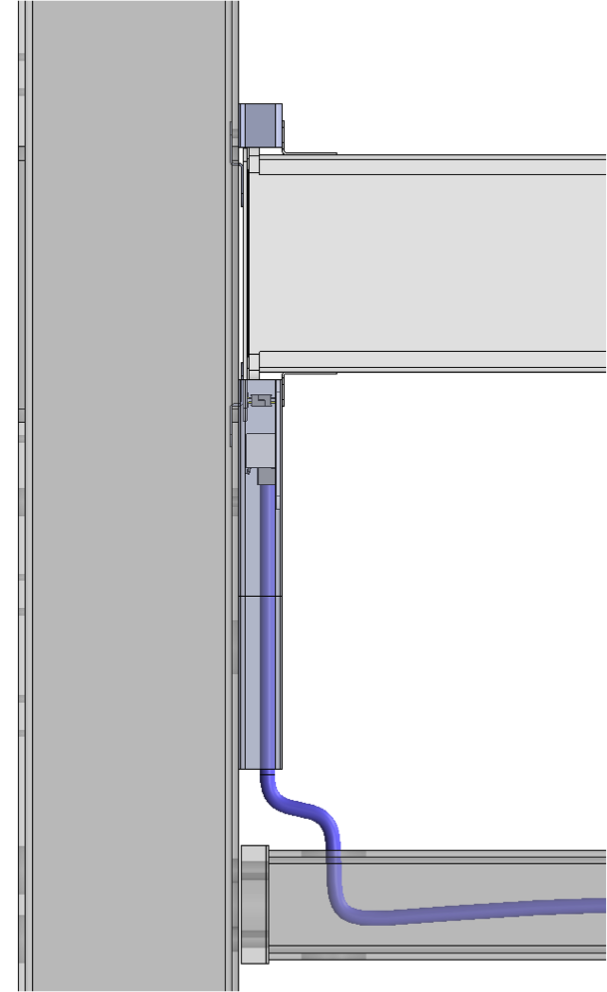
\includegraphics[height=0.3\textheight,trim=0mm 40mm 0mm 0mm,clip]{sp-apa-light-bar-cable.png}
\end{dunefigure}

As with the \dword{ce}, the interface between the \dword{pds} and \dwords{apa} involves a wide range of topics, including the hardware design and production, testing, integration, installation, and commissioning. 
%Depending on the final design of the \dword{pds}, the geometry of the \dword{apa}, including access slot dimensions, locations, and number, may require modification. Any proposed changes by the \dword{pds} consortium must be evaluated by the \dword{apa} consortium to consider structural effects or interference with other components.  
The electrical interface includes a grounding scheme and electrical insulation. The strict requirements on noise from the \dword{ce} means the electrical interface must be defined together with the \dword{sp} electronics consortium. 

For more information on the \dword{pds}, see Chapter~\ref{ch:fdsp-pd} % the Photon Detector Chapter in the \dword{tdr}.



%%%%%%%%%%%%%%%%%%%%%%%%%%%%%%%%%
\subsection{Cable Routing}
\label{sec:fdsp-apa-intfc-cables}

Cable routing schemes for both the \dword{tpc} electronics and \dword{pds} must be integrated into the design of the \dword{apa}s.   The \dword{ce} signal and power cables must be routed so that the head end of the lower \dword{apa} in the two-\dword{apa} assembly can be reached. \dword{ce} cables, therefore, will be routed inside the two side beams of the \dword{apa} frames. Figure~\ref{fig:apa-cable-tube} depicts such a cable routing scheme.  The \dword{ce} cables at the lower end of the lower \dword{apa} are formed into two bundles each about \SI{50}{mm} in diameter. Installation of the cables through the side tubes of the two stacked \dword{apa}s is done by pulling them through a large, smooth conduit placed inside each of the side tubes.  To fully accommodate the cables, the \dword{apa} frame hollow tube sections were enlarged relative to the \dword{pd} design from \SIrange{7.6}{10.2}{cm} (\SI{3}{in} to \SI{4}{in}) deep. Prototyping of this solution was carried out at PSL during summer 2018, as shown in the right photo in Figure~\ref{fig:apa-cable-tube}.     

%The \dword{ce} signal and power cables also must be routed so that the head end of the lower \dword{apa} in the two-\dword{apa} assembly can be reached. The current concept is to route the electronics cables inside the two side beams of the \dword{apa} frames. The right panel of Figure~\ref{fig:apa-cabling} depicts such a cable routing scheme. To fully accommodate the cables from two \dwords{apa}, we are considering using larger hollow tube sections. The final design is in progress, and prototyping is planned for later this year to verify a cabling and installation solution.     

\begin{dunefigure}[TPC electronics cable routing in the APAs]{fig:apa-cable-tube}
{Cable routing scheme. Left: Right: One of the cold electronics cable bundles being pulled through conduit of equal length to the two stacked \dword{apa}s.  The cable bundle is wrapped with a protective cover of braided PET plastic.  }
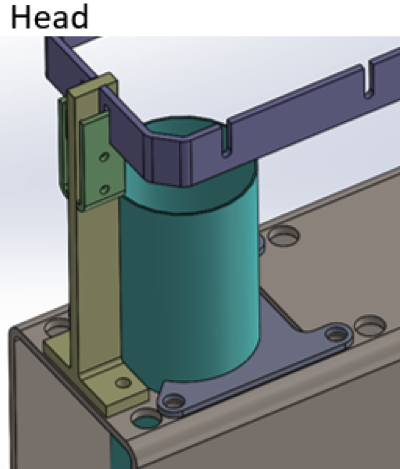
\includegraphics[height=0.3\textheight,trim=5mm 0mm 0mm 7mm,clip]{sp-apa-cable-tube-head.png} \quad
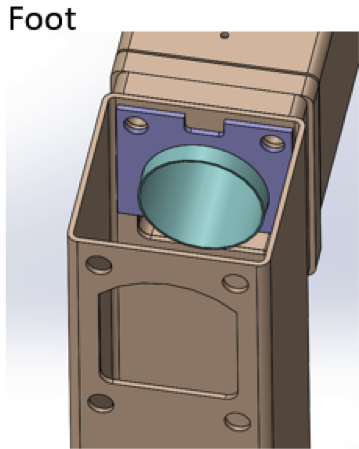
\includegraphics[height=0.3\textheight,trim=5mm 0mm 0mm 7mm,clip]{sp-apa-cable-tube-foot.png} \quad
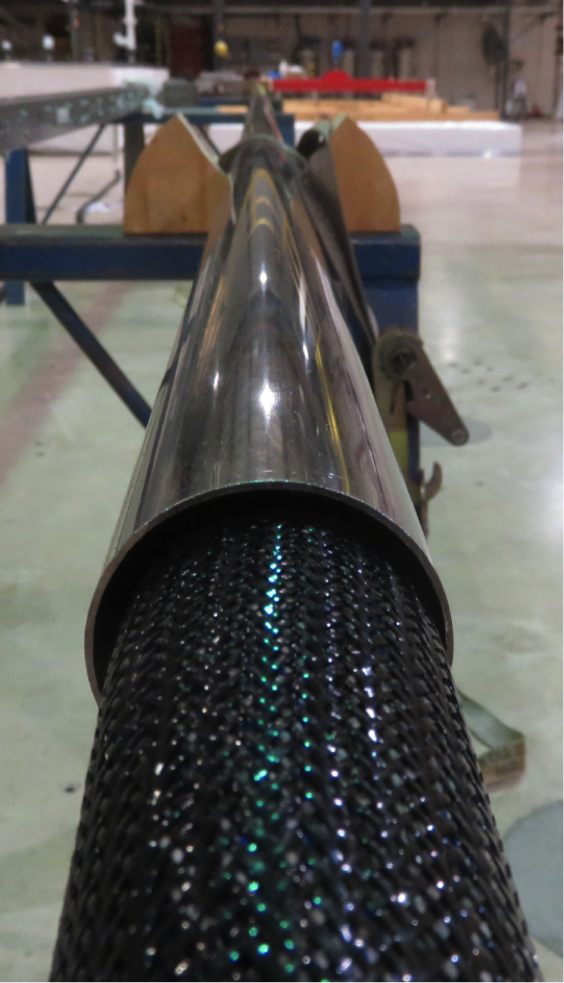
\includegraphics[height=0.3\textheight]{sp-apa-cable-tube-photo.png}
\end{dunefigure}

The concept being developed for the cables of the photon detectors is depicted in Figure~\ref{fig:apa-pds-cables}.  The cables run along the outside of the central tube in the \dword{apa} frame, joining together into a bundle of five cables by the time they reach the top of the frame.  Cables from the bottom \dword{apa} in a stack are fed through the foot tubes to the upper \dword{apa} and ran along the outside tubes on either side.  In this way, all \dword{pd} cables make it to the head of the upper \dword{apa}.  

\begin{dunefigure}[APA-to-APA connection and cable routing]{fig:apa-pds-cables}
{%Left: Conceptual design for the \dword{apa}-to-\dword{apa} connection.  The green insulator pieces act to electrically isolate the two frames as required by the \dword{fe} electronics.  Right: 
A concept for \dword{pds} cable routing. Top: The bottom \dword{apa}.  The \dwords{pd} are the ten transparent pieces spanning the frame -- two between each set of ribs.  They connect to their cables at the center tube.  The cables run up either side of the center tube (outside the tube) joining with others and forming two bundles of five cables by the time they reach the foot tube at the right end of this image. Middle: The top \dword{apa}. The two five-cable bundles from the lower \dword{apa} continue to the head tube of the upper \dword{apa} (at the right in this image) where they go through the head tube.  The cables from the \dwords{pd} in the upper \dword{apa} run up the outside of the center tube and form bundles which also go through the head tube. Bottom: Detail showing the five \dword{pds} cables gathered together at the foot tube (the top) of the bottom \dword{apa}.}
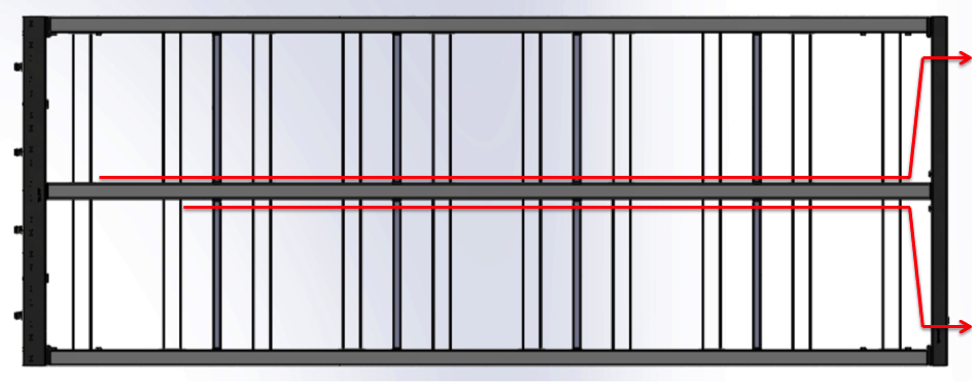
\includegraphics[width=0.78\textwidth]{sp-apa-pds-cables-bottom.png}
\hspace*{4mm}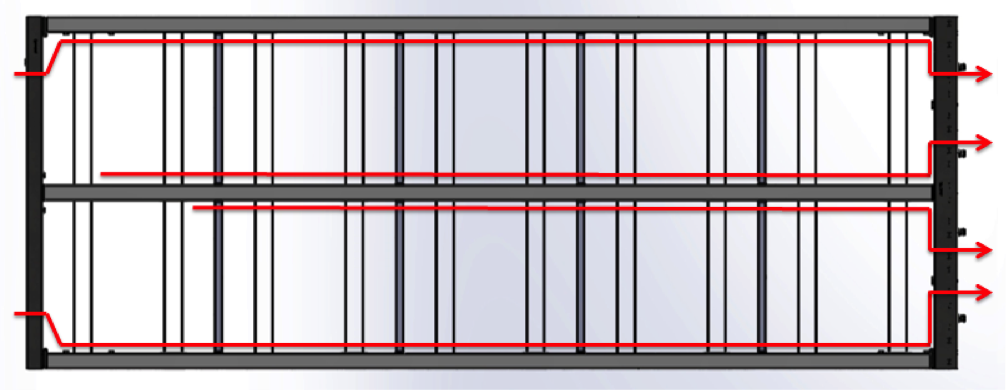
\includegraphics[width=0.8\textwidth]{sp-apa-pds-cables-top.png}
\vspace{5mm} \\
\hspace*{-10mm}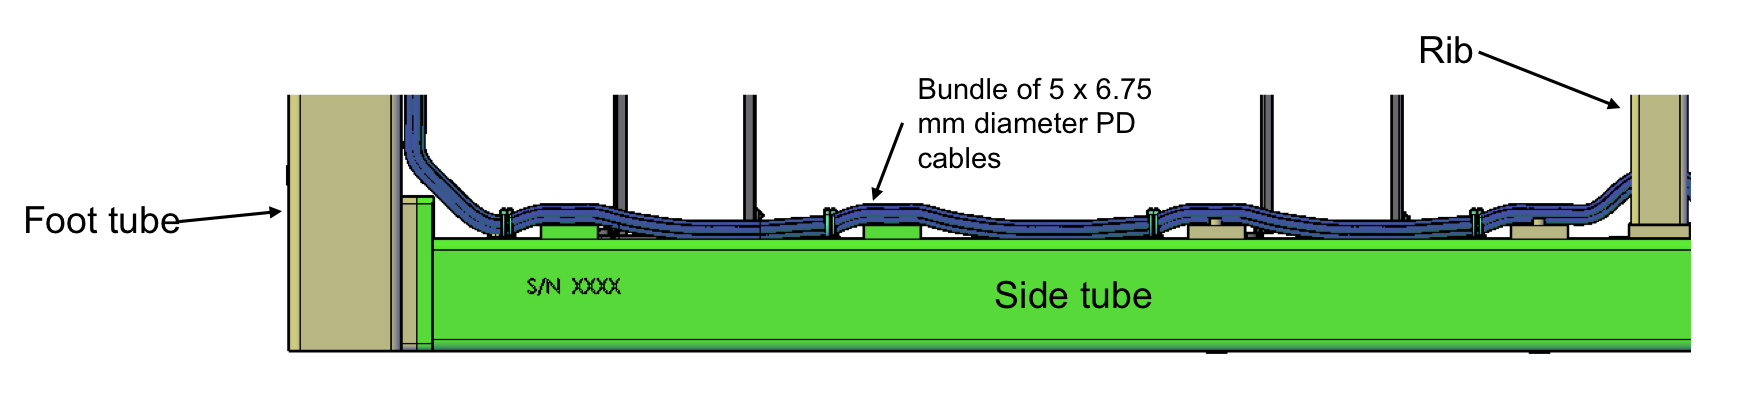
\includegraphics[width=0.9\textwidth]{sp-apa-pds-cables-detail.png}
%\setlength{\fboxsep}{0pt}
%\setlength{\fboxrule}{0.5pt}
%\fbox{\includegraphics[height=0.26\textheight]{apa-apa-mating.png}}\qquad \quad
%\includegraphics[height=0.26\textheight]{apa-cable-routing.png}
%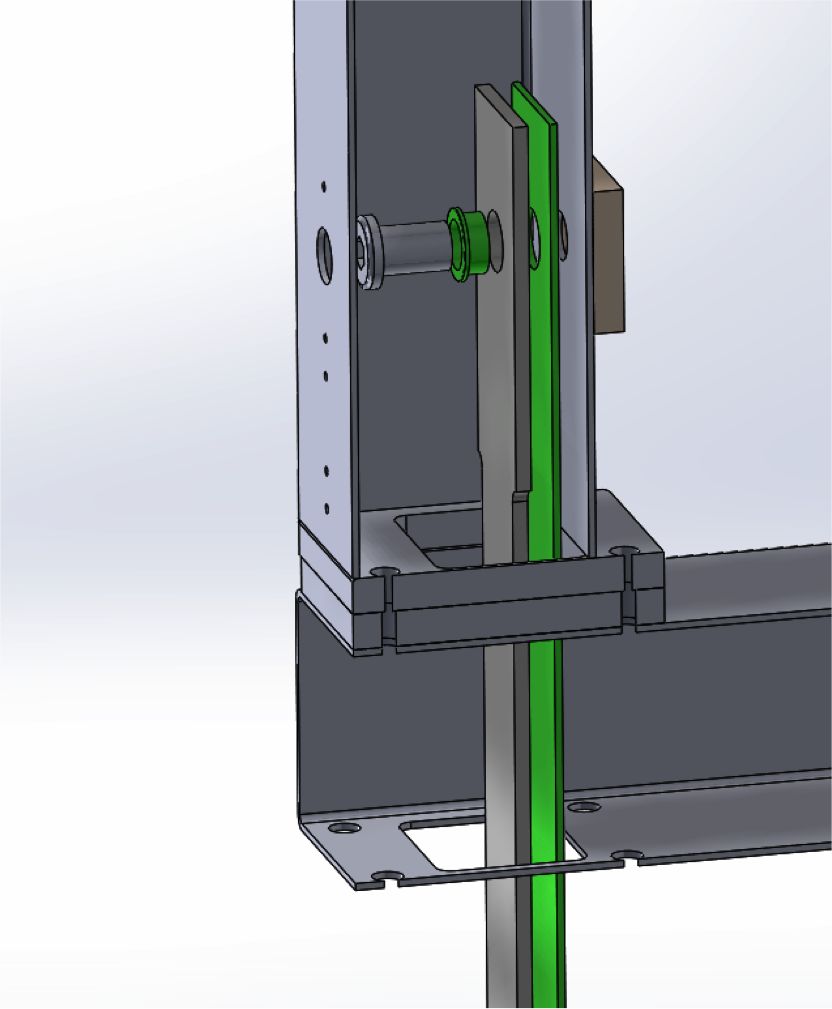
\includegraphics[height=0.26\textheight]{sp-apa-apa-mating.png} \qquad
%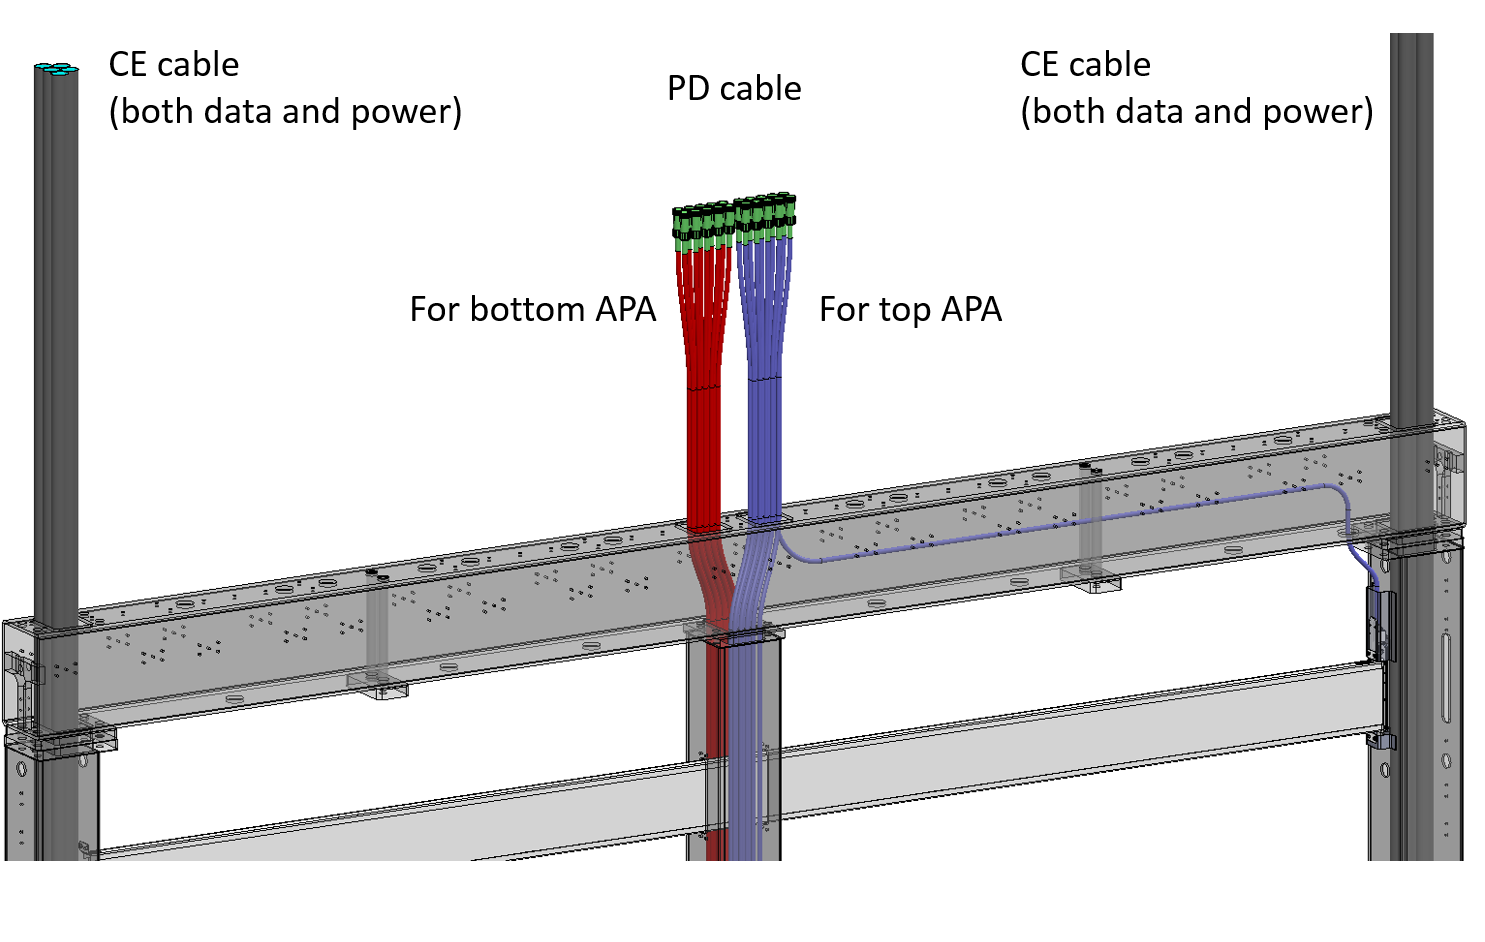
\includegraphics[height=0.35\textheight]{sp-apa-cable-routing.png}
\end{dunefigure}





